\section{Lec 6}
\subsection{Energy \& momentum}
Since out goal is to get to the Einstein Equation, we know that in there there should be the \emph{energy momentum tensor} $T^{\mu \nu }$. \\
As always we will study everything for a flat space-time but it will be useful for non flat ones. \\
We already saw the four-velocity $u^{\mu}$:
\[
u^{\mu } \equiv \frac{d x^{\mu }}{d\tau }
\]
while the proper time is $\Delta \tau^{2} = - \eta_{\mu \nu }dx^{\mu }dx^{\nu }$. \\
We need to make clear that we are talking about a time-like space-time trajectory, so $\Delta s^{2}<0$. \\
Let's start with the WL of a single particle, this is specified by a map $\mathbb{R}\to M$, where $M$ is a manifold that represents spacetime. We usually think the path as a curve parameterized by $\lambda $ so $x^{\mu }\left( \lambda  \right)$. \\
We also use as parameter the $\tau $ so $x^{\mu }\left( \tau  \right)$, this has some advantages because maybe it could be easier to switch to four-velocity.
\begin{equation}
u^{\mu }u_{\mu } = u_{\mu }u^{\mu } = \eta_{\mu \nu } u^{\mu }u^{\nu } = -1
\end{equation}
By the way, four-velocity is what we need to find the \emph{four momentum}:
\begin{equation}
p^{\mu } \equiv m u^{\mu }
\end{equation}
where m is the rest mass that has the same values $\forall$ RF, and it's just a number.

So in rest frame (x',y',z'):

\noindent
\begin{minipage}[t]{0.48\textwidth}
    \vspace*{0pt}
    

\tikzset{every picture/.style={line width=0.75pt}} %set default line width to 0.75pt        

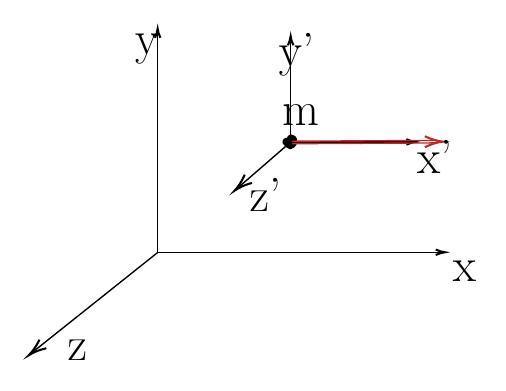
\begin{tikzpicture}[x=0.3pt,y=0.3pt,yscale=-1,xscale=1]
%uncomment if require: \path (0,514); %set diagram left start at 0, and has height of 514

%Straight Lines [id:da944915482116456] 
\draw    (250.32,299.23) -- (250.32,32) ;
\draw [shift={(250.32,30)}, rotate = 90] [color={rgb, 255:red, 0; green, 0; blue, 0 }  ][line width=0.75]    (10.93,-3.29) .. controls (6.95,-1.4) and (3.31,-0.3) .. (0,0) .. controls (3.31,0.3) and (6.95,1.4) .. (10.93,3.29)   ;
%Straight Lines [id:da15966795743012707] 
\draw    (250.32,299.23) -- (594.16,299.23) ;
\draw [shift={(596.16,299.23)}, rotate = 180] [color={rgb, 255:red, 0; green, 0; blue, 0 }  ][line width=0.75]    (10.93,-3.29) .. controls (6.95,-1.4) and (3.31,-0.3) .. (0,0) .. controls (3.31,0.3) and (6.95,1.4) .. (10.93,3.29)   ;
%Straight Lines [id:da1019518678879453] 
\draw    (250.73,299.23) -- (96.56,422.08) ;
\draw [shift={(95,423.32)}, rotate = 321.45] [color={rgb, 255:red, 0; green, 0; blue, 0 }  ][line width=0.75]    (21.86,-6.58) .. controls (13.9,-2.79) and (6.61,-0.6) .. (0,0) .. controls (6.61,0.6) and (13.9,2.79) .. (21.86,6.58)   ;
%Straight Lines [id:da7761915086395399] 
\draw    (410.52,166.36) -- (410.52,41) ;
\draw [shift={(410.52,39)}, rotate = 90] [color={rgb, 255:red, 0; green, 0; blue, 0 }  ][line width=0.75]    (10.93,-3.29) .. controls (6.95,-1.4) and (3.31,-0.3) .. (0,0) .. controls (3.31,0.3) and (6.95,1.4) .. (10.93,3.29)   ;
%Straight Lines [id:da2518341020035201] 
\draw    (410.52,166.36) -- (558.87,166.36) ;
\draw [shift={(560.87,166.36)}, rotate = 180] [color={rgb, 255:red, 0; green, 0; blue, 0 }  ][line width=0.75]    (10.93,-3.29) .. controls (6.95,-1.4) and (3.31,-0.3) .. (0,0) .. controls (3.31,0.3) and (6.95,1.4) .. (10.93,3.29)   ;
%Straight Lines [id:da6843037394854449] 
\draw    (410.7,166.36) -- (344.51,223.76) ;
\draw [shift={(343,225.07)}, rotate = 319.07] [color={rgb, 255:red, 0; green, 0; blue, 0 }  ][line width=0.75]    (21.86,-6.58) .. controls (13.9,-2.79) and (6.61,-0.6) .. (0,0) .. controls (6.61,0.6) and (13.9,2.79) .. (21.86,6.58)   ;
%Shape: Free Drawing [id:dp9557143063465285] 
\draw  [line width=3] [line join = round][line cap = round] (410.85,166.25) .. controls (410.85,167.51) and (410.44,163.59) .. (410.85,162.46) .. controls (411.44,160.78) and (416.94,165.75) .. (410.85,170.04) .. controls (409.05,171.31) and (407.47,166.25) .. (405.46,166.25) ;
%Straight Lines [id:da5108630624179767] 
\draw [color={rgb, 255:red, 192; green, 40; blue, 40 }  ,draw opacity=1 ]   (411.99,165.5) -- (585.99,164.54)(412.01,168.5) -- (586.01,167.54) ;
\draw [shift={(594,166)}, rotate = 179.69] [color={rgb, 255:red, 192; green, 40; blue, 40 }  ,draw opacity=1 ][line width=0.75]    (21.86,-6.58) .. controls (13.9,-2.79) and (6.61,-0.6) .. (0,0) .. controls (6.61,0.6) and (13.9,2.79) .. (21.86,6.58)   ;

% Text Node
\draw (219.7,32.51) node [anchor=north west][inner sep=0.75pt]   [align=left] {{\LARGE y}};
% Text Node
\draw (602.64,306.78) node [anchor=north west][inner sep=0.75pt]   [align=left] {{\LARGE x}};
% Text Node
\draw (138.58,401.86) node [anchor=north west][inner sep=0.75pt]   [align=left] {{\LARGE z}};
% Text Node
\draw (397,118) node [anchor=north west][inner sep=0.75pt]   [align=left] {{\LARGE m}};
% Text Node
\draw (392.97,31.76) node [anchor=north west][inner sep=0.75pt]   [align=left] {{\LARGE y'}};
% Text Node
\draw (559.44,161.51) node [anchor=north west][inner sep=0.75pt]   [align=left] {{\LARGE x'}};
% Text Node
\draw (357.7,206.48) node [anchor=north west][inner sep=0.75pt]   [align=left] {{\LARGE z'}};


\end{tikzpicture}

\end{minipage}
\begin{minipage}[t]{0.48\textwidth}
    \vspace*{0pt}
	So in the rest frame (x',y',z'): \\
   $p^{\mu }= \left( m,0,0,0 \right)$, because the \\four-velocity in the rest frame is \\$u^{\mu }= \left( 1,0,0,0 \right)$.  \\
   What is the expression of $p^{\mu }$ in the (x,y.z) frame?\\
   And what is the fastest way to compute it?		
\end{minipage}\hfill

We can start from the rest frame and use a LT. \\
For a generic four vector we have:
\begin{equation}
\begin{cases}
a^{0'} = \gamma \left( a^{0}- va^{1} \right) \\
a^{1'} = \gamma \left( a^{1}-va^{0} \right)\\
 a^{2'} = a^{2} \\
 a^{3'} = a^{3}
\end{cases}
\end{equation}
Now we find the inverse, we can search the inverse of the matrix or use an inverse LT,
\begin{equation}
\begin{cases}
a^{0} = \gamma \left( a^{0'}+va^{1'} \right) \\
a^{1} = \gamma \left( a^{1'}+va^{0'} \right) \\
a^{2} = a^{2'} \\
a^{3} = a^{3'}
\end{cases}
\end{equation}
So for the four-momentum we have:
\begin{equation}
\begin{cases}
	p^{0} = E = \gamma p^{0'} = \gamma m = \frac{m}{\sqrt{1-v^{2}}} \\
	p^{1} = m \gamma v = \frac{mv}{\sqrt{1-v^{2}}} \\
	p^{2} = 0 \\
	p^{3 }= 0
\end{cases}
\end{equation}
In the NR limit we should be able to recover Newton Mechanics:
\begin{gather*}
E  \approx m + \frac{mv^{2}}{2} + \ldots  \\
p^{1} \approx mv + \ldots 
\end{gather*}
The four-momentum as we got it provides the description of a single particle but often we need to study a lot of particles as a continuum, like a \emph{fluid}, characterized by quantities as density, pressure, entropy, viscosity... \\
A single momentum four-vector field is insufficient to describe the energy and the momentum of a fluid so we go further and define the \emph{energy-momentum tensor}.
\subsection{Energy-Momentum Tensor}
\[
T^{\alpha \beta }
\]
For now it is just a tensor, and we are happy to see that it transform like a tensor:
\[
T^{\alpha ' \beta '} = \Lambda^{\alpha '}_{\alpha }\Lambda^{\beta '}_{\beta }T^{\alpha \beta }
\]
In words, it is defined like "\emph{the flux of four-momentum $p^{\alpha }$ across the surface where $x^{\beta }$ is constant}".

For a system of \emph{N} particles we have: 
\[
p^{\alpha } = \sum_{j=1}^{N}{p^{\alpha }_{j}}	 
\]
where \emph{j} shows the \emph{j-th} particle, not an index to contract.
The \emph{number density, n} for a system of \emph{N} particles is:
\[
n = \sum_{j}^{}{\delta\left( \vec{r}-\vec{r}_{j} \right)}
\]
So we have these components of the energy-momentum tensor:
\begin{gather*}
T^{\alpha 0} = \sum_{j}^{}{p^{\alpha }_{j} \frac{dt}{dt} \delta\left( \vec{r}-\vec{r}_{j} \right)} \\
T^{\alpha i} = \sum_{j}^{}{p^{\alpha }_{j} \frac{dx^{i}_{j}}{dt} \delta\left( \vec{r}-\vec{r}_{j} \right) }
\end{gather*}
The $\frac{dt}{dt}$ is obvious that is simplified but we put it for clarity, while $ \frac{dx^{i}_{j}}{dt} $ is the flux.
The meaning is that the tensor is the output of many contribution, each contribute has the center around the \emph{j-th} particle.

This gives me all the components of the E-M tensor. Now, what is a tensor? We used the word tensor because we know a priori what we are gonna find it, but without knowing and looking at the definition and components. We will do it by looking at LTs, and how they act on this object.

First thing we compute:
\[
\frac{ dx^{i}_{j}}{dt} = \frac{ dx^{i}_{j}}{d\tau } \colorbox{yellow}{$ \frac{d\tau }{dt}$} = \frac{dx^{i}_{j}}{d\tau } \colorbox{yellow}{$ \frac{1}{\gamma_{j}}$}
\]
because
\[
\frac{d\tau ^{2}}{dt^{2}} = \frac{dt^{2}-dx^{2}}{dt^{2}} = 1 - v^{2}_{j} = \frac{1}{\gamma^{2}_{j}}
\]
why is it useful? Because it appears in components
\[
\frac{dx^{i}_{j}}{d\tau } = \left( m^{j} \frac{dx^{i}_{j}}{d\tau } \right) \frac{1}{m_{j}\gamma_{j}} = \frac{p^{i}_{j}}{p^{0}_{j}}		
\]
so i can rewrite the energy-momentum tensor like:
\[
T^{\alpha \beta } = \sum_{j}^{}{\frac{ p^{\alpha }_{j}p^{\beta }_{j}}{p^{0}_{j}}\delta\left( \vec{r}-\vec{r}_{j} \right)}
\]
so if 
\begin{itemize}
	\item $\beta =0 \to p^{\alpha }_{j}$ 
	\item $\beta =1 \to \frac{p^{i}_{j}}{p^{0}_{j}}$
\end{itemize}
If i switch $\alpha $ with $\beta $, I find the same objects, because the tensor is symmetric.
\[
	T^{\left( \alpha \beta  \right)} = T^{\alpha \beta } \text{  ;   } T^{[\alpha \beta ]} = 0
\]
Why is a tensor? If I change frame I can change 

If I change frame I have to change $\alpha , \beta $ but also $p_{0}$ that is not Lorentz Invariant, It's the energy of the particle \emph{j}, and with a boost it will be different.\\
We have shown that 
\[
\frac{\delta\left( \vec{r}-\vec{r}_{j} \right)}{p^{0}_{j}}
\]
is a Lorentz scalar. 
Writing
\[
T^{\alpha \beta }_{j}= \frac{p^{\alpha }_{j}p^{\beta }_{j}}{p^{0}_{j}} \delta^{\left( 3 \right)}\left( \vec{r}-\vec{r}_{j} \right) 
\]
with a 3-d Dirac Delta function, and with this definition 
\[
T^{\alpha  \beta } = \sum_{j}^{}{T^{\alpha \beta }_{j}}
\]
that is a tensor because sum of tensors is still a tensor.

Let's focus on the single contribution:
\begin{gather*}
T^{\alpha \beta }_{j} = \frac{p^{\alpha }_{j} m u^{\beta }_{j}}{m \gamma_{j}} \delta^{\left( 3 \right)}\left( \vec{r}-\vec{r}_{j} \right) =\\
\end{gather*}
we see that $m u^{\beta }$ is $p^{\beta }$, and $m \gamma $ is $p^{0}$. We can simplify the masses and we get:
\begin{gather*}
T^{\alpha \beta }_{j} = \frac{p^{\alpha }_{j} u^{\beta }_{j}}{ \gamma_{j}} \delta^{\left( 3 \right)}\left( \vec{r}-\vec{r}_{j} \right) =\\
= \int_{}^{}{d\tau_{j} p^{\alpha }_{j} u^{\beta }_{j} \delta^{\left( 4 \right)}\left( x^{\mu }-x^{\mu }_{j}\left( \tau_{j} \right) \right)} =
\end{gather*}
The two expression are equivalent, to show it I have to compute the integral. I use the delta function of the 0 component: so the \emph{p,u, $\gamma $} elements can be extracted from the integral and we compute just
\begin{equation}
	= \int_{}^{}{d\tau_{j} \delta\left( x^{0}-x^{0}_{j}\left( \tau  \right) \right)} = \int_{}^{}{\frac{1}{\left| \frac{dx^{0}_{j}}{d\tau }\right|_{d\overline{\tau }}} d\tau_{j} \delta\left( \tau_{j}-\overline{\tau_{j}} \right)}= 
\end{equation}
$\overline{\tau }$ is where the argument of the delta function is 0. The integral is straightforward. We have to change variable of the delta function, that gets contributes only from the point that match the argument, I integrate $\tau_{j} - \text{ number }$, There is a jacobian factor: $\frac{1}{\left| \frac{dx^{0}_{j}}{d\tau }\right|_{d\overline{\tau }}}$ that is equal to $\gamma_{j} = \frac{dt}{d\tau_{j}}$.

This is a tensor, because I have objects with indices $\alpha, \beta $, integral over $\tau_{j}$ which is a Lorentz Invariant Scalar and a $\delta $ over all space coordinates.

Delta function has the very useful property:
\begin{gather*}
\delta\left( f\left( x \right) \right) = \frac{1}{\left| f'\left( x_{0} \right)\right|} \delta\left( x-x_{0} \right) \to \int_{x-\epsilon }^{x+\epsilon }{dx \delta \left( x-x_{0} \right)}=1\\
\end{gather*}

\subsubsection{Case I: Dust}
The dust is defined as \emph{generic ensemble of N particles that move very slowly}. So it's any set of particles with kinetic energy much smaller than rest mass energy.

SO the important part is that the relative velocity in some RF $\to 0$.

The total energy density $\rho $ is described as 
\[
	T^{00} = \sum_{j = 1}^{N}{p^{0}_{j} \delta\left( x- \overline{x}_{j} \right)} = \rho 
\]
So dust in the rest frame is 
\begin{equation}
T^{\mu \nu }\begin{pmatrix}
m\cdot n & 0 & 0 & 0 \\
0 & 0 & 0 & 0 \\
0 & 0 & 0 & 0 \\
0 & 0 & 0 & 0
\end{pmatrix} 
\end{equation}
where $\rho = m\cdot n$, all particles have the same mass, $n$ is the number density. It's clear that if the particles are at rest, the flux is null.

What is $T^{\mu \nu }$ in a generic frame? I could apply LTs, (and we are invited to try it), but actually i can reason a little on the meaning of the tensor.

I can call $u^{\mu }$ \emph{fluid four-velocity}, if you think about that there is a velocity field on a moving fluid like a river. In the rest frame
\[
u^{\mu }= \left( 1,0,0,0 \right)
\]
so 
\[
T^{\mu \nu } = \rho u^{\mu }u^{\nu }
\]
This is more generic way to find the tensor $T^{\mu \nu }$ in a generic frame, The strategy, as you may guess, is that I know the expression in a generic frame and I want to recover the tensor from this.

Dust is something very common in cosmology, and is a fluid with zero pressure. But is not always true that in a fluid the pressure is negligible. Photons for example do not have 0 pressure or relative velocity $\to 0$.

\subsubsection{Case II: Fluid with pressure or \emph{Perfect FLuid} }

Be
\begin{equation}
T^{\mu \nu }_{rest} = \begin{pmatrix}
\rho  & 0 & 0 & 0 \\
0 & p & 0 & 0 \\
0 & 0 & p & 0 \\
0 & 0 & 0 & p
\end{pmatrix} 
\end{equation}

Let's talk about the physics underlying this definition: \\
The parts $0i$ or $i0$ under rotations or LTs transform like \emph{3-d} vectors, and since the values are 0s, the fluid is \emph{isotropic} $\to $ no preference about any direction.\\
\emph{ij} parts represent the flux of momentum \emph{p} against surface of constant spatial coordinates. Momentum flux is the force, and force flux is the pressure. We could have different $p_{i}$ along the diagonal, the fluid wouldn't be isotropic, but there will still be 0 sheer forces.

In the most generic frame:
\begin{equation}
T^{\mu \nu } = \rho u^{\mu }u^{\nu }+ p \eta^{\mu \nu } + p u^{\mu } u^{\nu } = \left( \rho +p \right) u^{\mu }u^{\nu } + p \eta^{\mu \nu }
\end{equation}

\subsubsection{Conservation of energy and momentum}
$p^{\mu _{ \text{ total }}}$ has to be constant, so energy and momentum are constant.
I want this condition to be local:
\[
p^{\mu }_{ \text{ total } } = \int_{V}^{}{dx^{3}T^{\mu 0}} = \int_{4d}^{}{dS_{\nu }T^{\mu \nu }}
\]
If i set $\nu =0$ I simplify it. I integrate over the entire $V$ that is the entire space. It can be written as the flux of the $\nu $ components. The four dimensional integral has a surface $S$ where $T^{\mu \nu }$ is constant. It's a flux integral. $dS_{\nu } = \left( 1,0,0,0 \right)$.

\[
\Delta p^{\mu }_{ \text{ total }} = p^{\mu }_{ \text{ total }}\left( t_{2} \right) - p^{\mu }_{ \text{ total }}\left( t_{1} \right)
\]
So let's make a scheme to understand the situation.

\noindent
\begin{minipage}[t]{0.48\textwidth}
    \vspace*{0pt}
\tikzset{every picture/.style={line width=0.5pt}} %set default line width to 0.75pt       
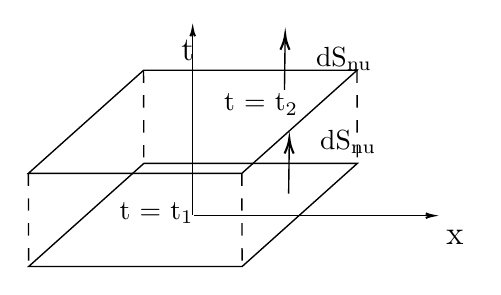
\begin{tikzpicture}[x=0.25pt,y=0.25pt,yscale=-1,xscale=1]
%uncomment if require: \path (0,514); %set diagram left start at 0, and has height of 514

%Straight Lines [id:da944915482116456] 
\draw    (250.32,299.23) -- (250.32,32) ;
\draw [shift={(250.32,30)}, rotate = 90] [color={rgb, 255:red, 0; green, 0; blue, 0 }  ][line width=0.75]    (10.93,-3.29) .. controls (6.95,-1.4) and (3.31,-0.3) .. (0,0) .. controls (3.31,0.3) and (6.95,1.4) .. (10.93,3.29)   ;
%Straight Lines [id:da15966795743012707] 
\draw    (252.32,300.23) -- (596.16,300.23) ;
\draw [shift={(598.16,300.23)}, rotate = 180] [color={rgb, 255:red, 0; green, 0; blue, 0 }  ][line width=0.75]    (10.93,-3.29) .. controls (6.95,-1.4) and (3.31,-0.3) .. (0,0) .. controls (3.31,0.3) and (6.95,1.4) .. (10.93,3.29)   ;
%Shape: Rectangle [id:dp13264483463125742] 
\draw   (179.7,224.73) -- (488.23,224.73) -- (321.76,373.73) -- (13.23,373.73) -- cycle ;
%Shape: Rectangle [id:dp5241947086840221] 
\draw   (179.29,90.11) -- (487.82,90.11) -- (321.35,239.11) -- (12.82,239.11) -- cycle ;
%Straight Lines [id:da9873328008653245] 
\draw    (383,118.5) -- (383.98,40.5) ;
\draw [shift={(384,38.5)}, rotate = 90.72] [color={rgb, 255:red, 0; green, 0; blue, 0 }  ][line width=0.75]    (21.86,-6.58) .. controls (13.9,-2.79) and (6.61,-0.6) .. (0,0) .. controls (6.61,0.6) and (13.9,2.79) .. (21.86,6.58)   ;
%Straight Lines [id:da7100914300813527] 
\draw    (389,268.5) -- (389.98,190.5) ;
\draw [shift={(390,188.5)}, rotate = 90.72] [color={rgb, 255:red, 0; green, 0; blue, 0 }  ][line width=0.75]    (21.86,-6.58) .. controls (13.9,-2.79) and (6.61,-0.6) .. (0,0) .. controls (6.61,0.6) and (13.9,2.79) .. (21.86,6.58)   ;
%Straight Lines [id:da5752286958121103] 
\draw  [dash pattern={on 4.5pt off 4.5pt}]  (12.82,239.11) -- (13.23,373.73) ;
%Straight Lines [id:da3625750970621462] 
\draw  [dash pattern={on 4.5pt off 4.5pt}]  (179.29,90.11) -- (179.7,224.73) ;
%Straight Lines [id:da36524075127919386] 
\draw  [dash pattern={on 4.5pt off 4.5pt}]  (487.82,90.11) -- (488.23,224.73) ;
%Straight Lines [id:da5000478553674463] 
\draw  [dash pattern={on 4.5pt off 4.5pt}]  (321.35,239.11) -- (321.76,373.73) ;

% Text Node
\draw (219.7,32.51) node [anchor=north west]   [align=left] {{\large t}};
% Text Node
\draw (602.64,306.78) node [anchor=north west]   [align=left] {{\large x}};
% Text Node
\draw (266,267) node [anchor= north east]   [align=left] {{ t = t\textsubscript{1}}};
% Text Node
\draw (268,110) node [anchor=north west]   [align=left] {{ t = t\textsubscript{2}}};
% Text Node
\draw (401,43) node [anchor=north west]   [align=left] {{ dS\textsubscript{nu}}};
% Text Node
\draw (407,193) node [anchor=  west]   [align=left] {{ dS\textsubscript{nu}}};
\end{tikzpicture}
\end{minipage}
\begin{minipage}[t]{0.48\textwidth}
    \vspace*{0pt} 
    This is an integral of the flux along the time direction. \par
    So the expression of $\Delta p^{\mu }_{ \text{ total }}$ can be written as \par
\end{minipage}

\[
= \int_{ \text{ total surface }}^{}{dS_{\nu }T^{\mu \nu }} = \int_{Volume}^{}{dx^{3}\partial_{\nu }T^{\mu \nu }} = \int_{volume}^{}{dV \partial_{\nu }T^{\mu \nu }}
\]
So we have two surfaces and we closed it inside a solid, and it is like we are doing gauss theorem, We can use the divergence theorem in 4d. We state that the divergence of $T^{\mu \nu }$:
\begin{gather*}
\partial_{\mu }T^{\mu \nu } = 0 \\
\partial_{\nu }T^{\mu \nu } = 0
\end{gather*}
And that's a way to express conservation.

\paragraph{Results for perfect fluids}
\[
T^{\mu \nu } = \left( \rho  +p \right) u^{\mu }u^{\nu }+p \eta^{\mu \nu }
\]
and taking the derivative
\begin{gather*}
\partial_{\mu } T^{\mu \nu } = \partial_{\mu }\left( \rho +p \right)u^{\mu }u^{\nu } + \partial_{\mu }p \eta^{\mu \nu } + \left( \rho +p \right)\left( \partial_{\mu }u^{\mu } \right)u^{\nu } + \left( \rho +p \right) u^{\mu }\partial_{\mu }u^{\nu } = \\
= \partial_{\mu }\left( \rho +p \right)u^{\mu }u^{\nu }+ \partial_{\mu }p \eta^{\mu \nu } + \left( \rho +p \right) [\left( \partial_{\mu }u^{\mu }u^{\nu } + u^{\mu }\partial_{\mu }u^{\nu } \right)]
\end{gather*}
It is quite clear, just the thing that we neglect derivative of the metric because in flat spacetime it is a constant matrix, and so it's 0.\par
Let's take the projection of this identity along the direction of the four-velocity.
\begin{gather*}
	u_{\nu }\partial_{\mu }T^{\mu \nu } = -\partial_{\mu }\left( \rho +p \right)u^{\mu }+\left( \partial_{\mu }p \right)u^{\mu }+\left( \rho +p \right)[-\partial_{\mu }u^{\mu }+u_{\nu }u^{\mu }\partial_{\mu }u^{\nu }] =
\end{gather*}
and since, 
\[
\partial_{\mu }\left( u_{\nu }u^{\nu } \right) = 0 = \partial_{\mu }\left( -1 \right)
\]
we get
\begin{equation}
= -\partial_{\mu }\left( \rho +p \right)u^{\mu } + \partial_{\mu }p u^{\mu }- \left( \rho +p \right)\partial_{\mu }u^{\mu } = 0
\end{equation}
And in the NR limit, $p\ll \rho $:
\begin{gather*}
-\partial_{\mu }\rho  u^{\mu }+\rho \partial_{\mu }u^{\mu }+ \partial_{\mu }pu^{\mu }=0 \\
\text{ we can neglect the last term since the hypothesis } \\
\partial_{\mu }\left( \rho u^{\mu } \right) = 0 \implies \partial_{t}\rho +\partial_{i}\left( \rho u^{i} \right) = 0
\end{gather*}
we recover the continuity equation.

\paragraph{exercise}: instead of projecting on $u^{\nu  }$, project orthogonal to $u^{\mu }$,compute: $p^{\alpha }_{\nu } \partial_{\mu }T^{\mu \nu }=0$.
idk what it means: $p^{\alpha }_{\beta }\equiv \delta^{\alpha }_{\beta } + u^{\alpha }u_{\beta }$. Evaluate alpha = 1,2,3.





